\documentclass[lettersize,journal]{IEEEtran}

% ------------------------------------------------------------
% Dwell indexed robust invariant sets for safe weathervaning
% station keeping. Target journal IEEE/ASME T-Mech.
% Draft of 2026-10-14. Builds without any figure file present.
% Prose deliberately avoids colons, semicolons, hyphens and
% dashes. Math, the \thanks block, bib entries and LaTeX
% syntax are exempt.
% ------------------------------------------------------------

\usepackage{amsmath,amssymb,amsthm}
\usepackage{bm}
\usepackage{booktabs}
\usepackage{makecell}
\usepackage{graphicx}
\usepackage{xcolor}
\usepackage{cite}
\usepackage{algorithm}
\usepackage{algorithmic}
\usepackage{url}

% Placeholders. \pending renders red, \figph draws a boxed placeholder.
\newcommand{\pending}[1]{\textcolor{red}{[#1]}}
\newcommand{\figph}[2]{\fbox{\parbox[c][#2][c]{0.94\linewidth}{\centering\footnotesize\textcolor{red}{#1}}}}

% Theorem environments (author convention, bracketed names)
\newtheorem{definition}{Definition}
\newtheorem{assumption}{Assumption}
\newtheorem{lemma}{Lemma}
\newtheorem{proposition}{Proposition}
\newtheorem{theorem}{Theorem}
\newtheorem{remark}{Remark}
\renewcommand{\qedsymbol}{$\blacksquare$}

% Author biography with photo, \biography{file in figures/}{name}{text}
\newcommand{\biography}[3]{\IfFileExists{figures/#1}%
{\begin{IEEEbiography}[{\includegraphics[width=1in,height=1.25in,clip,keepaspectratio]{figures/#1}}]{#2}#3\end{IEEEbiography}}%
{\begin{IEEEbiographynophoto}{#2}#3\end{IEEEbiographynophoto}}}

\newcommand{\calA}{\mathcal{A}}
\newcommand{\calW}{\mathcal{W}}
\newcommand{\calS}{\mathcal{S}}
\newcommand{\calT}{\mathcal{T}}
\newcommand{\gR}{\mathrm{R}}
\newcommand{\gN}{\mathrm{N}}
\newcommand{\gF}{\mathrm{F}}

\begin{document}

\title{Safe Weathervaning of an Autonomous Surface Vessel Under Gear Shift Dwell via Dwell Indexed Robust Invariant Sets}

\author{Kiyong~Park and Jinwhan~Kim,~\IEEEmembership{Member,~IEEE}%
\thanks{Manuscript received XXXX; revised XXXX. (Corresponding author: Jinwhan Kim.)}%
\thanks{The authors are with the Department of Mechanical Engineering, Korea Advanced Institute of Science and Technology (KAIST), Daejeon 34141, Republic of Korea (e-mail: qkrrldyd777@gmail.com; jinwhan@kaist.ac.kr).}}

\markboth{IEEE/ASME Transactions on Mechatronics}%
{Park and Kim, Safe Weathervaning Station Keeping Under Gear Shift Dwell}

\maketitle

\begin{abstract}
This article presents a dwell indexed robust invariant set framework for the safe weathervaning station keeping of a small autonomous surface vessel driven by a single engine and a sterndrive, which holds station by letting its bow align with the environmental load. However, the gear shift must hold each of the reverse, neutral, and forward positions for a minimum dwell time, and since sterndrive steering vectors the thrust, a lock in neutral removes thrust and steering authority, a constraint that existing controllers and safety certificates treat nominally or ignore. The central observation is that the dwell binds only the control player of the zero sum safety game while the disturbance acts at every instant, so the safe set is a family indexed by the elapsed dwell. The gear state and its timer are promoted to state variables, the augmented game is shown to preserve the discounted safety backup, and the dwell indexed value is learned by a one step adversarial backup with legality masking. A task policy trained under the certified value and a value threshold shield complete the controller. Simulations expose the false certification of a dwell unaware certificate, and full scale field experiments against PID and nonlinear model predictive baselines show the real disturbance lying inside the certified bound, so that the certified margin acts as a reserve.
\end{abstract}

\begin{IEEEkeywords}
Autonomous surface vessels, dwell time, robust invariant sets, safe reinforcement learning, station keeping, sterndrive.
\end{IEEEkeywords}

\section{Introduction}\label{sec_intro}

\IEEEPARstart{S}{mall} autonomous surface vessels (ASVs) are increasingly deployed for hydrographic survey, water quality sampling, harbor inspection, and passenger transport in confined waters \cite{liu2016,shi2017,lee2024canal}. Many of these missions contain phases in which the vessel must hold a position rather than follow a path. A survey boat waits at a station until a sensor cast is complete, a canal boat waits in front of a lock or a berth until it is cleared to proceed, and a rendezvous requires the vessel to loiter around a point until a partner arrives. For a small vessel with a single engine and a sterndrive this station keeping is most naturally performed by weathervaning. The position is held inside a region around the setpoint while the heading is left free, so that the bow aligns with the resultant wind and current load and the vessel holds station with the actuation it has, as in the weather optimal positioning of Fossen and Strand \cite{fossen2001wopc} and the underactuated positioning of Pettersen and Fossen \cite{pettersen2000underactuated}.

The sterndrive that makes such a vessel inexpensive also makes the task difficult, and the difficulty is mechatronic rather than hydrodynamic. The engine drives the propeller through a gearbox with reverse, neutral, and forward positions, and for the mechanical reasons explained in Section~\ref{sec_dwell} the shift must hold each position for a minimum dwell of about three seconds. During that time the controller cannot change the sign of the thrust, and since a sterndrive steers by vectoring the propeller thrust, a lock in neutral leaves the vessel with neither thrust nor steering authority. Wind and current do not wait for the lock to expire.

Station keeping controllers for marine craft range from proportional integral derivative (PID) and line of sight designs \cite{yu2022los} to nonlinear model predictive control (NMPC) with identified vessel models \cite{lee2024canal}. When a discrete actuator must respect a minimum dwell, the model predictive literature on switched systems offers mixed integer and dwell constrained formulations \cite{zhang2016,vicente2019,lavaei2021,zhuang2023,chenlazar2022}. However, these results are either nominal or linear. The switched tube constructions of \cite{zhang2016,vicente2019,lavaei2021} tighten constraints against additive disturbances for linear dynamics only, the persistent dwell results of \cite{zhuang2023} are stated for linear switched systems, and the nonlinear scheme of \cite{chenlazar2022} establishes recursive feasibility through an $\ell$ step control invariant terminal set without a tightening mechanism for disturbances. In addition, all of these works treat the dwell as a design output that guarantees stability or feasibility, whereas on a sterndrive the dwell is a hardware constant and the question is where the vessel may operate so that it survives the locks the hardware will impose.

Safety against bounded disturbances is naturally posed as a two player zero sum reachability game \cite{bansal2017}, and recent learning based methods compute its value for nonlinear systems that are beyond grid based solvers. The discounted safety backup of Fisac et al. \cite{fisac2019}, reachability constrained reinforcement learning \cite{yu2022}, its adversarial extension by Li et al. \cite{li2023cdc,li2309dual}, decomposition based safety filters \cite{li2311decomp}, and DeepReach \cite{bansal2021deepreach} all deliver a value function whose zero superlevel set is a robust invariant set (RIS). However, every one of them assumes that the full control set is available at every step, so none models an actuator that locks. The exact computation of disturbance invariant sets under a dwell time restriction by Dehghan and Ong \cite{dehghan2012} is the closest predecessor of the present work, but it is confined to linear polytopic dynamics, quantifies universally over disturbance sequences, and returns a binary membership verdict that no shield can threshold.

In this article, the dwell is reinterpreted not as a scheduling restriction but as an asymmetry of the safety game. The dwell binds only the maximizing player, and the disturbance remains free at every step. As a consequence the safe set is not one set but a family indexed by the elapsed dwell. The gear state and its timer are therefore promoted to the state, and the dwell indexed value is learned by a one step adversarial backup in which legality is enforced both in the plant and in the backup. The learned value drives a task policy and a safety shield, and the complete controller is validated in simulation against a dwell unaware certificate and in full scale field experiments against PID and NMPC baselines. To the best of our knowledge, this study represents the first field demonstration of a learned robust safety certificate on a full scale vessel subject to a physical actuator dwell. The main contributions of this article are summarized as follows.
\begin{enumerate}
\item A dwell indexed robust invariant set is formulated for weathervaning station keeping, in which the gear state and its elapsed dwell are promoted to state variables and the safe set becomes a family indexed by the elapsed dwell, in contrast to the single sets of \cite{dehghan2012,zhang2016,vicente2019} and to the dwell free certificates of \cite{fisac2019,li2023cdc}.
\item A one step adversarial learning scheme with legality masking is developed for the dwell indexed value on the identified nonlinear vessel model, together with a task policy and a value threshold shield that use the learned value as a scalar margin at run time.
\item Full scale field experiments on an eight meter sterndrive vessel are conducted against PID and NMPC baselines, and a simulation study exposes the false certification produced when the dwell is ignored.
\end{enumerate}

The remainder of this article is organized as follows. Section~\ref{sec_system} describes the vessel, the physical origin of the shift dwell, the maneuvering model, and the disturbance model. Section~\ref{sec_problem} formulates the augmented safety game and establishes that the augmentation preserves its structure. Section~\ref{sec_method} develops the dwell indexed safe controller, its learning scheme, the task policy, and the shield. Section~\ref{sec_results} presents the system identification, simulation, and field results, including the onboard implementation. Section~\ref{sec_conclusion} concludes this article, and the proof of the lemma is given in the Appendix. Fig.~\ref{fig_framework} shows the overall framework.

\begin{figure*}[!t]
\centering
\IfFileExists{figures/fig_framework.pdf}{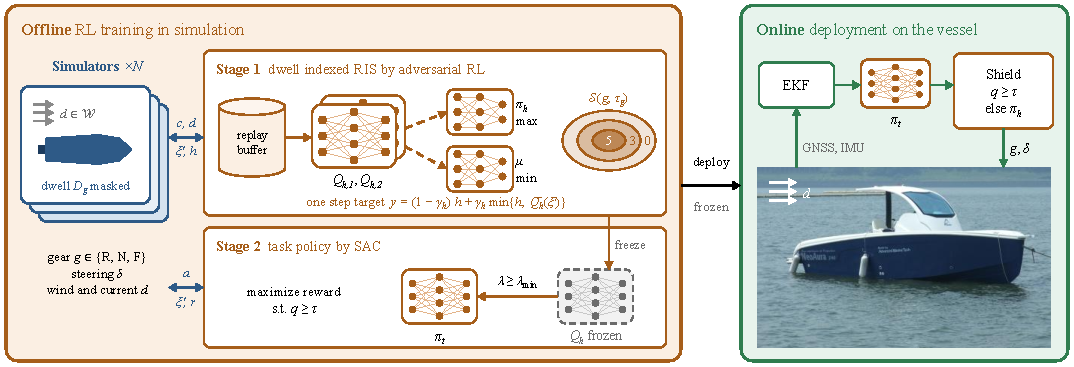
\includegraphics[width=\textwidth]{figures/fig_framework.pdf}}{\figph{Fig. 1 placeholder. Overall framework.}{5cm}}
\caption{Overall framework of the proposed dwell indexed safe station keeping. Offline, parallel simulators that enforce the gear dwell fill a replay buffer, from which the twin safety critics $Q_{h,1}$ and $Q_{h,2}$ are learned by a one step adversarial game between the safety policy $\pi_h$ and the adversary $\mu$ (Stage~1), and the task policy $\pi_t$ is trained by soft actor critic under the frozen safety critic (Stage~2). Online, the frozen networks run on the vessel at each control period, and the shield replaces the task action by $\pi_h$ whenever the certified value falls below the margin $\tau$.}
\label{fig_framework}
\end{figure*}

\section{System Description and Modeling}\label{sec_system}

This section describes the vessel and its actuation, explains where the gear shift dwell comes from, and presents the vehicle dynamics model used for training together with the disturbance model. The presentation follows the modeling practice of \cite{lee2024canal} and the model class of \cite{fossen2011}.

\subsection{Vessel and Actuation System}\label{sec_vessel}

The experimental platform is a Neo AURA 240 EXP with a deep V planing hull, propelled by a single inboard diesel engine \pending{model} driving a MerCruiser Bravo~1 sterndrive, and shown in Fig.~\ref{fig_vessel}(a) with the GPS antenna on the T top and the attitude and heading reference system (AHRS) and the control PC, a laptop computer running ROS~2, at the console. Three actuation channels are exposed to the controller through the chain shown in Fig.~\ref{fig_vessel}(b). The engine speed is commanded over a CAN interface, while the gear shift among reverse, neutral, and forward and the steering angle of the drive are executed by two electric linear servo cylinders, one acting on the shift cable and one mounted on the drive pivot, both driven by an LS XGB programmable logic controller (PLC) through an EtherCAT servo interface. A bow thruster is installed on the vessel but is not used in this study, so that the results concern a single engine sterndrive configuration, and the specifications of the platform and its sensors are listed in Table~\ref{tab_boat}.

\begin{figure*}[!t]
\centering
\IfFileExists{figures/fig_vessel.pdf}{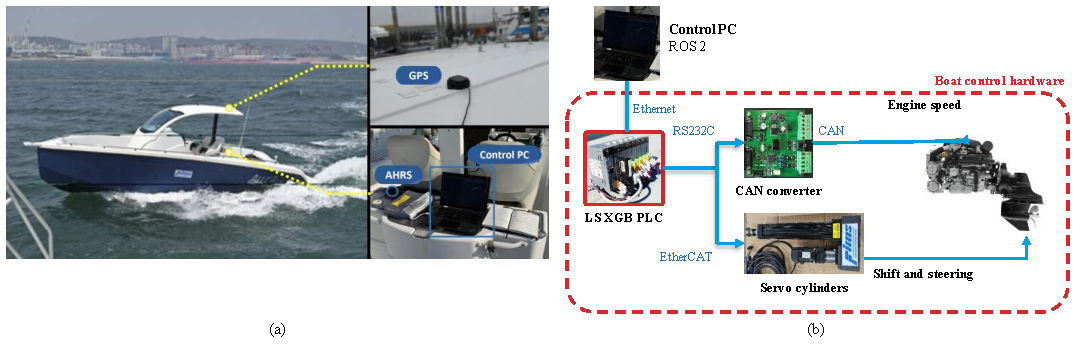
\includegraphics[width=\textwidth]{figures/fig_vessel.pdf}}{\figph{Fig. 2 placeholder. Vessel with sensors and control hardware.}{5cm}}
\caption{Experimental vessel and its hardware. (a) The vessel with the GPS antenna, the AHRS, and the control PC. (b) Control hardware connected to the control PC of (a) by Ethernet, from the PLC to the engine and the sterndrive, with the communication interface of each link.}
\label{fig_vessel}
\end{figure*}

\subsection{Gear Shift Dwell}\label{sec_dwell}

The minimum dwell has a mechanical origin that the controller cannot shorten. A shift between forward and reverse passes through neutral, and the cone clutch of the sterndrive gearbox must engage at low engine speed to avoid shock loading of the gear set. The shift cylinder therefore first brings the engine to idle, moves its stroke to the new detent, and only then releases the engine speed command \pending{confirm this shift sequence against the PLC logic of the vessel}. The elapsed time of this sequence, together with a protection interval that prevents an immediate reversal of the stroke, sets the minimum interval between consecutive shift commands. On the vessel of this study this interval is 3~s \pending{measured basis, cylinder stroke time and protection interval to be stated}. With the control period of 0.5~s the dwell corresponds to $D_g = 6$ control steps. A shift request issued during the dwell is not delayed but discarded by the plant, so the controller must reason about when it is allowed to act.

\subsection{Vehicle Dynamics Modeling}\label{sec_model}

The vessel is described by the three degree of freedom horizontal plane model of \cite{fossen2011} in the body fixed and inertial frames of Fig.~\ref{fig_frames}, written in the form used in \cite{lee2024canal} as
\begin{subequations}\label{eq_model}
\begin{align}
M\dot{\nu} + C(\nu)\nu + D(\nu)\nu &= \bm{f}_c + M d, \\
\dot{\eta} &= R(\psi)\nu, \\
R(\psi) &= \begin{bmatrix} \cos\psi & -\sin\psi & 0 \\ \sin\psi & \cos\psi & 0 \\ 0 & 0 & 1 \end{bmatrix},
\end{align}
\end{subequations}
where $\nu = [u, v, r]^\top$ and $\eta = [x, y, \psi]^\top$ are the velocity and position vectors, respectively, $M$ is the inertia matrix, $C(\nu)$ is the Coriolis and centripetal matrix, $D(\nu)$ is the damping matrix, $\bm{f}_c = [f_X, f_Y, f_N]^\top$ represents the control forces and moment in each direction, $d = [d_u, d_v, d_r]^\top$ is the disturbance acceleration bounded in \eqref{eq_wbox}, and $R(\psi)$ is the rotation matrix from the body fixed frame to the inertial frame. The control vector is denoted $\bm{f}_c$ rather than $\tau_c$ because $\tau$ is reserved for the shield margin and $\tau_g$ for the dwell timer in this article. Assuming that the vessel is symmetric in the $x$ and $y$ directions, $M$, $C(\nu)$, and $D(\nu)$ can be expressed as
\begin{equation}
M = \operatorname{diag}(m_{11}, m_{22}, m_{33}),
\label{eq_mass}
\end{equation}
\begin{equation}
C(\nu) = \begin{bmatrix} 0 & 0 & -m_{22} v \\ 0 & 0 & m_{11} u \\ m_{22} v & -m_{11} u & 0 \end{bmatrix},
\label{eq_coriolis}
\end{equation}
\begin{equation}
D(\nu) = -\begin{bmatrix} X_u & 0 & 0 \\ 0 & Y_v & Y_r \\ 0 & N_v & N_r \end{bmatrix}
- \begin{bmatrix} X_{u|u|}|u| & 0 & 0 \\ 0 & Y_{v|v|}|v| & Y_{r|r|}|r| \\ 0 & N_{v|v|}|v| & N_{r|r|}|r| \end{bmatrix},
\label{eq_damping}
\end{equation}
where $m_{11}$, $m_{22}$, and $m_{33}$ are the mass and moment of inertia including the added mass and added moment of inertia, $X_u$, $Y_v$, $Y_r$, $N_v$, and $N_r$ are the linear drag coefficients, and $X_{u|u|}$, $Y_{v|v|}$, $Y_{r|r|}$, $N_{v|v|}$, and $N_{r|r|}$ are the nonlinear drag coefficients, respectively.

The control force and moment are produced by the propeller thrust vectored through the steering angle of the drive,
\begin{equation}
\bm{f}_c = \begin{bmatrix} f_X \\ f_Y \\ f_N \end{bmatrix}
= \begin{bmatrix} F_g\cos\delta \\ F_g\sin\delta \\ -l_d F_g\sin\delta \end{bmatrix},
\label{eq_force}
\end{equation}
where $F_g$ is the propeller thrust at gear level $g \in \{\gR, \gN, \gF\}$ at the throttle setting used in this study, with $F_{\gN} = 0$ and $F_{\gR} < 0 < F_{\gF}$, $\delta$ is the steering angle of the drive, and $l_d$ is the distance from the origin of the body fixed frame to the drive. In \cite{lee2024canal} the outboard thrust is commanded continuously through the throttle as $F = c\,n_T^2$, whereas here the thrust takes only the three values selected by the gear, and the gear is the channel that carries the dwell. Since the lateral force $f_Y$ and the yaw moment $f_N$ are proportional to $F_g$, both vanish together with the thrust in neutral. The steering angle moves toward its command $\delta_c$ at no more than the slew rate of the servo cylinder, which over an integration substep of length $\Delta t_s$ reads
\begin{equation}
\delta^{+} = \delta + \operatorname{sat}_{\dot{\delta}_{\max}\Delta t_s}\!\bigl(\delta_c - \delta\bigr), \qquad |\delta_c| \le \delta_{\max},
\label{eq_steer}
\end{equation}
with the angle limit $\delta_{\max}$ and the rate limit $\dot{\delta}_{\max}$ matched to the servo cylinder \pending{values}. Combining \eqref{eq_model} to \eqref{eq_force} without the disturbance, the complete model is written as
\begin{equation}
\dot{\bm{x}} = f(\bm{x}, \bm{u}, P),
\label{eq_complete}
\end{equation}
where $\bm{x} = [x, y, \psi, u, v, r]^\top$ and $\bm{u} = [g, \delta_c]^\top$ are the state and control input vectors, respectively, and $P = [m_{11}, m_{22}, m_{33}, X_u, Y_v, Y_r, N_v, N_r, X_{u|u|}, Y_{v|v|}, Y_{r|r|}, N_{v|v|}, N_{r|r|}, F_{\gF}, F_{\gR}, l_d]$ is the vector of unknown parameters. \pending{confirm that the training simulator integrates \eqref{eq_model} including $C(\nu)$, since the earlier simulator code omitted the Coriolis term}

\begin{figure}[!t]
\centering
\IfFileExists{figures/fig_frames.pdf}{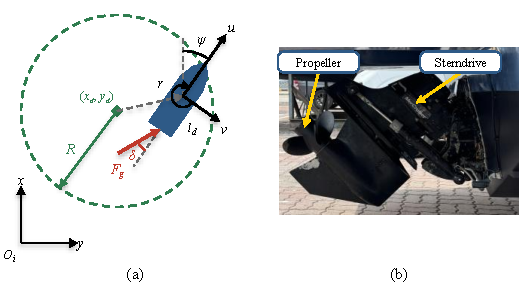
\includegraphics[width=0.6\linewidth]{figures/fig_frames.pdf}}{\figph{Fig. 3 placeholder. Coordinate frames and sterndrive geometry.}{4cm}}
\caption{Coordinate frames and sterndrive geometry. Inertial and body fixed frames, the keep in disk of radius $R$ around the setpoint, and the thrust $F_g$ vectored by the steering angle $\delta$ at the distance $l_d$ behind the origin.}
\label{fig_frames}
\end{figure}

The environmental load is represented by a body frame acceleration $d = [d_u, d_v, d_r]^\top$ that enters \eqref{eq_model} through the term $Md$ and is bounded by the box
\begin{equation}
\calW = [-\bar{d}_u, \bar{d}_u] \times [-\bar{d}_v, \bar{d}_v] \times [-\bar{d}_r, \bar{d}_r].
\label{eq_wbox}
\end{equation}
The bounds are chosen from drift data recorded on the vessel with the engine at idle and the gear in neutral, in which the measured accelerations reflect the wind and current load alone. The bounds are set to cover the recorded drift with a margin \pending{bounds $\bar d_u$, $\bar d_v$, $\bar d_r$ and the recording conditions}. No assumption is made on the time behavior of $d$ within $\calW$. In the safety game of Section~\ref{sec_problem} the disturbance is chosen by an adversary at every step, which is a stronger model than any particular wind spectrum.

\section{Problem Formulation}\label{sec_problem}

This section promotes the gear state and its timer to state variables, defines the legality structure that the dwell induces, and establishes that the resulting augmented game retains the structure required by the discounted safety backup.

\subsection{Why Dwell Breaks the Markov Property}

Consider two situations with identical physical states. In the first, the gear was shifted three seconds ago, so any gear command is admissible now. In the second, it was shifted half a second ago, so no gear command is admissible for the next two and a half seconds. Identical states, different admissible action sets. The process is therefore not Markov in the physical state alone, and a value function learned on it conflates the two situations. The remedy is to promote the relevant past into the state.

\subsection{Augmented State and Legal Action Set}

Let $(\tilde{x}, \tilde{y}) = (x - x_d, y - y_d)$ be the position error from the setpoint $(x_d, y_d)$ and let $\tilde{\psi}$ be the heading relative to a fixed reference, which is kept in the state for the dynamics but is unconstrained by the task. Let $\tau_g \in \{0, 1, \ldots, D_g - 1\}$ denote the remaining lock time of the shift in control steps, with $\tau_g = 0$ meaning that the gear may be shifted now. The augmented state is
\begin{equation}
\xi = (\tilde{x}, \tilde{y}, \tilde{\psi}, u, v, r, \delta, g, \tau_g) \in \Xi,
\label{eq_xi}
\end{equation}
and the control is $c = (\delta_c, g_c)$ with the steering command $\delta_c \in \calA_\delta = [-\delta_{\max}, \delta_{\max}]$ and the gear command $g_c$. The legal action set is the product
\begin{equation}
C(\xi) = \calA_\delta \times C_g(g, \tau_g), \qquad
C_g = \begin{cases} \{g\}, & \tau_g > 0,\\ \{\gR, \gN, \gF\}, & \tau_g = 0, \end{cases}
\label{eq_legal}
\end{equation}
so that the steering channel carries no dwell while the gear channel is locked whenever its timer is positive. Whenever the gear switches to a new level its timer resets to $D_g - 1$, and otherwise the timer counts down toward zero. Holding the current gear is always legal, so $C(\xi)$ is nonempty, and it is compact as a product of a finite set and a compact interval. The augmented transition $\xi' = F(\xi, c, d)$ consists of the physical map obtained by integrating \eqref{eq_model} and \eqref{eq_steer} over one control period under the legal gear, together with the timer update.

\begin{definition}[Dwell Constrained Admissible Policy]\label{def_admissible}
A policy $\pi \colon \Xi \to \calA_\delta \times \{\gR, \gN, \gF\}$ is dwell constrained admissible if $\pi(\xi) \in C(\xi)$ for every $\xi \in \Xi$. The set of such policies is denoted $\Pi_C$.
\end{definition}

\begin{remark}[Masking Lives in Two Places]\label{rem_masking}
The legality structure \eqref{eq_legal} must be enforced in two distinct places. First, in the plant, where a shift request issued during a lock is ignored and the current gear is held, exactly as the PLC does on the vessel. Second, in the backup of Section~\ref{sec_game}, where the maximization must range over $C(\xi)$ and not over the full action set. It is tempting to omit the second enforcement and expect a neural network to learn the restriction from data. If the approximation error lets the learned value believe that a locked gear can correct immediately, the fixed point certifies safety that does not exist. The failure is optimistic rather than conservative, and Section~\ref{sec_sim_a1} exhibits it.
\end{remark}

\subsection{The Augmented Safety Game}\label{sec_game}

The task is encoded by the keep in function
\begin{equation}
h(\xi) = R - \sqrt{\tilde{x}^2 + \tilde{y}^2},
\label{eq_h}
\end{equation}
whose zero superlevel set is the disk of radius $R$ around the setpoint. The function depends only on the position error, so the heading is free and the vessel may weathervane. On the augmented state the safety value function is defined by
\begin{equation}
V_h^{*}(\xi) = \max_{\pi \in \Pi_C} \min_{\mu} \min_{k \ge 0} h(\xi_k),
\label{eq_value}
\end{equation}
where $\mu$ ranges over nonanticipative disturbance strategies with values in $\calW$ \cite{bansal2017}. The value is the best worst margin achievable from $\xi$ under legally restricted control, and $\{\xi \mid V_h^{*}(\xi) \ge 0\}$ is the largest set on which the vessel can remain inside the disk forever against every admissible disturbance. The undiscounted self consistency condition of \eqref{eq_value} is not a contraction. Fisac et al. introduced a discount $\gamma_h \in (0,1)$ that restores contraction \cite{fisac2019}, and the device was extended to the disturbed game by Li et al. \cite{li2023cdc}. The resulting backup on the augmented state is
\begin{equation}
(\calT_h V)(\xi) = (1-\gamma_h) h(\xi) + \gamma_h \min\Bigl\{ h(\xi),\ \max_{c \in C(\xi)} \min_{d \in \calW} V\bigl(F(\xi, c, d)\bigr) \Bigr\},
\label{eq_backup}
\end{equation}
which differs from the operator of \cite{li2023cdc} only in that the maximization ranges over the state dependent legal set. The following lemma states that nothing else changes.

\begin{lemma}[Preservation of the Game Structure]\label{lem_aug}
Let the augmented dynamics follow \eqref{eq_xi} and \eqref{eq_legal}, let $h$ be bounded, and let $\calT_h$ be defined by \eqref{eq_backup}. Then $\calT_h$ is a monotone $\gamma_h$ contraction in the supremum norm, it admits a unique bounded fixed point $V_h$, and the set $\calS = \{\xi \mid V_h(\xi) \ge 0\}$ is a robust invariant set of the augmented system under dwell constrained admissible policies.
\end{lemma}

The proof is given in the Appendix. In plain terms, the lemma says that the dwell does not damage the mathematical machinery, because the contraction argument uses only the fact that the admissible action set is nonempty and compact at every state. All difficulty introduced by the dwell is therefore concentrated not in the operator but in the shape of its fixed point, which the next section examines.

\begin{remark}[Several Dwell Channels]\label{rem_channels}
The formulation extends to $N$ independent switching channels, each with its own levels, dwell constant, and timer, by taking $C(\xi)$ as the product of the per channel legal sets, and Lemma~\ref{lem_aug} holds verbatim since no step of its proof counts the channels. Only the gear channel is treated in this article.
\end{remark}

\section{Dwell Indexed Safe Controller}\label{sec_method}

This section contains the conceptual core of the article. We first show that the safe set under the dwell is a family indexed by the elapsed dwell and locate its physical origin in the asymmetry between control and disturbance on a sterndrive. We then describe the one step learning of the dwell indexed value and the task policy and shield built on it.

\subsection{The Safe Set Is a Family Indexed by Elapsed Dwell}\label{sec_family}

Fix the discrete coordinates of the augmented state and consider the slice of the RIS over the physical coordinates,
\begin{equation}
\calS(g, \tau_g) = \bigl\{ (\tilde{x}, \tilde{y}, \tilde{\psi}, u, v, r, \delta) \mid V_h(\xi) \ge 0 \bigr\}.
\label{eq_family}
\end{equation}
Each choice of gear and timer produces a different slice, so the safe set is a family indexed by the elapsed dwell. The dependence is monotone in the natural direction. When $\tau_g = 0$ the gear can react immediately and the slice is large. When $\tau_g = D_g - 1$ the vessel must survive the entire lock without gear authority, so the margin that the disturbance can erode during the lock must be reserved in advance and the slice is small. Fig.~\ref{fig_family} illustrates the slices.

The physical origin of the family is an asymmetry in the game \eqref{eq_value}. The dwell binds only the maximizing player. On a sterndrive the asymmetry is particularly severe, because steering vectors the thrust. During a lock in neutral the propeller produces no thrust and, by \eqref{eq_force}, no lateral force and no yaw moment either, so the control authority is exactly zero for up to three seconds. During a lock in forward or reverse the vessel can steer but cannot reverse its thrust, so a vessel that has just engaged forward to climb back toward the setpoint cannot brake if the wind pushes it across. Throughout those seconds the disturbance acts freely at every step. In a zero sum game, tying one player's hands lowers the value, and the amount by which the value drops is exactly the amount by which the safe set shrinks. The adversary of \eqref{eq_value} does not need a larger disturbance to exploit this. It needs the right timing, namely the moments at which the gear has just been locked in the wrong level. The dwell indexed value function anticipates this timing because the timer is part of its argument, whereas a dwell unaware value cannot.

\begin{figure}[!t]
\centering
%\includegraphics[width=\linewidth]{figures/fig_family.pdf}
\figph{Fig. 5 placeholder. Slices of the certified set in the position error plane for each gear level (rows R, N, F) and selected timer values (columns, timer 0, 2, 5), at a representative heading and velocity. Keep in circle of radius R drawn on each panel. The slice shrinks with the timer, most strongly for the neutral gear.}{5.5cm}
\caption{The safe set is a family indexed by the gear level and the elapsed dwell. Slices of the certified set over the position error for fixed heading and velocity. A larger remaining lock reserves more margin and yields a smaller slice, and the neutral lock produces the smallest slices. \pending{Generated from the trained value, to be inserted.}}
\label{fig_family}
\end{figure}

\subsection{One Step Learning of the Dwell Indexed Value}\label{sec_learning}

The fixed point of \eqref{eq_backup} is learned by a one step adversarial actor critic scheme in the lineage of reachability constrained reinforcement learning \cite{yu2022} and its disturbed extension \cite{li2023cdc}, adapted to the legality structure. Algorithm~\ref{alg_ris} summarizes the procedure. The network input encodes the augmented state as
\begin{equation}
\bigl(\tilde{x}/R,\ \tilde{y}/R,\ \sin\tilde{\psi},\ \cos\tilde{\psi},\ u,\ v,\ r,\ \delta/\delta_{\max},\ \operatorname{onehot}(g),\ \tau_g/D_g\bigr),
\label{eq_input}
\end{equation}
so that the gear and the timer are visible to every network.

\subsubsection{Safety Critics}
Two safety critics $Q_{h,1}(\xi, c, d)$ and $Q_{h,2}(\xi, c, d)$ with target copies $\bar{Q}_{h,1}$ and $\bar{Q}_{h,2}$ approximate the value of the joint action and disturbance, and the minimum of the two is used everywhere a critic value is needed. For a transition $(\xi, c, d, \xi')$ drawn from the replay buffer the regression target is
\begin{equation}
y = (1-\gamma_h) h(\xi) + \gamma_h \min\Bigl\{ h(\xi),\ \min_{i} \bar{Q}_{h,i}\bigl(\xi', \pi_h(\xi'), \mu(\xi')\bigr) \Bigr\},
\label{eq_target}
\end{equation}
where $\pi_h$ is the protagonist and $\mu$ the adversary described below. Since $h$ is bounded above by $R$, the bootstrap term is clipped to the physical value range $[-h_{\mathrm{floor}}, R]$, and $h$ itself is floored at $-h_{\mathrm{floor}}$ outside the disk so that the value remains bounded as Lemma~\ref{lem_aug} requires. The critics are regressed onto $y$ by a squared loss, and the target copies follow the critics by a soft update.

\subsubsection{Protagonist}
The protagonist $\pi_h$ outputs a Gaussian steering command squashed by $\tanh$ to $\calA_\delta$ and sampled by the reparameterization trick, together with a categorical distribution over the gear levels in which the illegal levels of $C_g(g, \tau_g)$ are masked to zero probability. Writing $q(\xi, c) = \min_i Q_{h,i}(\xi, c, \mu(\xi))$ for the minimum critic at the adversary's disturbance, it is trained to maximize the exact expectation of $q$ over the legal discrete actions,
\begin{equation}
J_\pi = \mathbb{E}_{\xi}\Bigl[ \sum_{g' \in C_g(g,\tau_g)} p_\pi(g' \mid \xi)\ \mathbb{E}_{\delta' \sim \pi_h(\cdot \mid \xi)}\bigl[ q\bigl(\xi, (\delta', g')\bigr) \bigr] \Bigr],
\label{eq_actor}
\end{equation}
which enumerates the at most three legal gear levels instead of sampling them and therefore removes the variance of a sampled discrete action.

\subsubsection{Adversary}
The adversary $\mu(\xi)$ is a deterministic policy whose output is scaled by $\tanh$ into the box $\calW$, and it is trained to minimize the minimum critic at the protagonist's action. During data collection exploration noise is added to the adversary so that the replay buffer contains disturbance realizations around the current worst case rather than only at it.

\subsubsection{Curricula and Coverage}
Two curricula stabilize the game. The adversary scale is ramped from zero to one, so that the protagonist first learns to hold station in calm water and then faces a progressively stronger opponent, and the discount $\gamma_h$ is ramped from 0.95 to 0.995, so that the horizon of the certificate grows as the value estimate improves. At every episode reset the full augmented state is randomized, including the gear level and the timer, so that states entered in the middle of a lock are covered by data even though they cannot be chosen by the protagonist.

\begin{algorithm}[!t]
\caption{One Step Learning of the Dwell Indexed Value}
\label{alg_ris}
\begin{algorithmic}[1]
\STATE Initialize critics $Q_{h,1}, Q_{h,2}$, targets $\bar{Q}_{h,1}, \bar{Q}_{h,2}$, protagonist $\pi_h$, adversary $\mu$, replay buffer $\mathcal{B}$, adversary scale $\kappa \gets 0$, discount $\gamma_h \gets 0.95$
\FOR{each episode}
\STATE Sample $\xi_0$ uniformly over $\Xi$, including $g$ and $\tau_g$
\FOR{each step $k$}
\STATE $c_k \gets$ sample from $\pi_h(\cdot \mid \xi_k)$ with illegal gear levels masked
\STATE $d_k \gets \kappa\,\mu(\xi_k) +$ exploration noise, projected onto $\calW$
\STATE $\xi_{k+1} \gets F(\xi_k, c_k, d_k)$ with the plant ignoring illegal shift requests
\STATE Store $(\xi_k, c_k, d_k, \xi_{k+1})$ in $\mathcal{B}$
\STATE Sample a minibatch from $\mathcal{B}$ and form $y$ by \eqref{eq_target} with clipping
\STATE Update $Q_{h,1}, Q_{h,2}$ by regression onto $y$
\STATE Update $\pi_h$ by ascending \eqref{eq_actor} over the legal gear levels
\STATE Update $\mu$ by descending $\min_i Q_{h,i}(\xi, \pi_h(\xi), \mu(\xi))$
\STATE Soft update $\bar{Q}_{h,i} \gets (1-\rho)\bar{Q}_{h,i} + \rho Q_{h,i}$
\ENDFOR
\STATE Advance the curricula $\kappa \to 1$ and $\gamma_h \to 0.995$
\ENDFOR
\end{algorithmic}
\end{algorithm}

\subsubsection{Certified and Deployed Sets}
After training, the certified set is
\begin{equation}
\hat{\calS} = \bigl\{ \xi \mid q\bigl(\xi, \pi_h(\xi)\bigr) \ge 0 \bigr\},
\label{eq_certified}
\end{equation}
and the deployed set is the margin shifted level set $\hat{\calS}_\tau = \{\xi \mid q(\xi, \pi_h(\xi)) \ge \tau\}$ with a margin $\tau > 0$ calibrated by adversarial Monte Carlo audit as described in Section~\ref{sec_sim_audit}.

\begin{remark}[Scope of the Guarantee and the Margin]\label{rem_scope}
Contraction, uniqueness, and invariance hold at the operator level. The value is represented by neural networks, and no bound on the approximation error is claimed here. Moreover, since $\gamma_h < 1$, the zero level set of the discounted fixed point is optimistic relative to the undiscounted value \eqref{eq_value}. The deployed certificate is therefore the shifted level set $\hat{\calS}_\tau$, whose margin $\tau$ absorbs both the approximation error and the discount optimism, and every certified rate reported in this article refers to this audited level set rather than to $\hat{\calS}$.
\end{remark}

\subsection{Task Policy and Safety Shield}\label{sec_shield}

With the safety critics, the protagonist, and the adversary frozen, a task policy $\pi_t$ is trained by soft actor critic \cite{haarnoja2018} in a second stage. The reward combines the distance to the setpoint, a term that favors keeping a gear engaged over idling in neutral, a steering effort term, and a penalty on each intervention of the shield,
\begin{equation}
r_t = -w_1 \sqrt{\tilde{x}^2 + \tilde{y}^2} - w_2\, \mathbf{1}[g = \gN] - w_3\, \delta_c^2 - w_4\, \mathbf{1}[\text{shield active}],
\label{eq_reward}
\end{equation}
with weights $w_1$ to $w_4$ \pending{values}. The task actor has the same masked output structure as the protagonist, so it never requests an illegal shift. Safety enters the second stage as a Lagrangian penalty on the certified value,
\begin{equation}
\max_{\pi_t}\ \mathbb{E}\bigl[ Q_t(\xi, \pi_t(\xi)) \bigr] + \lambda\, \mathbb{E}\bigl[ \min\{0,\ q(\xi, \pi_t(\xi)) - \tau\} \bigr],
\label{eq_lagrange}
\end{equation}
where $Q_t$ is the task critic, $q$ is the frozen minimum safety critic of Section~\ref{sec_learning}, and the multiplier $\lambda$ is adapted by dual ascent but floored at a positive minimum $\lambda_{\min} > 0$ so that the safety pressure never vanishes even when the constraint is inactive. The floor is what keeps the task policy inside the deployed set during training instead of letting it drift to the boundary of the certificate.

At run time the two policies are combined by a value threshold filter. At each control step the task action $c^{t} = \pi_t(\xi)$ is evaluated by the frozen critic, and the applied action is
\begin{equation}
c = \begin{cases} c^{t}, & q(\xi, c^{t}) \ge \tau, \\ \pi_h(\xi), & \text{otherwise}, \end{cases}
\label{eq_shield}
\end{equation}
so that the safety policy takes over only when the task action would leave the deployed set under the worst disturbance. The filter uses the same networks and the same margin as the certificate. \pending{Exact onboard switching rule to be confirmed against the deployed code, including whether the filter evaluates the task action alone or also the hold action.}

\section{Simulation and Experimental Results}\label{sec_results}

The effectiveness of the proposed approach is validated through numerical simulation and full scale field experiments. The vessel model of Section~\ref{sec_model} is first identified from experimental data, simulations are then conducted with the identified model to audit the certificate and to compare the closed loop behavior against the baselines, and field experiments on the vessel follow.

\subsection{System Identification Results}\label{sec_si_results}

\begin{table}[!t]
\renewcommand{\arraystretch}{1.3}
\caption{Boat Specifications}
\label{tab_boat}
\centering
\footnotesize
\begin{tabular}{ll}
\toprule
\multicolumn{2}{l}{(a) Platform specification} \\
\midrule
Hull & Neo AURA 240 EXP, deep V planing hull \\
Length overall & 8.29 m \\
Length between perpendiculars & 6.96 m \\
Breadth & 2.62 m \\
Depth & 0.66 m \\
Draft & 0.34 m \\
Capacity & 12 persons \\
Engine & single inboard diesel, \pending{model} \\
Minimum shift dwell & 3 s, \pending{measured basis} \\
\midrule
\multicolumn{2}{l}{(b) Sensor specification} \\
\midrule
RTK GPS & \makecell[l]{ZED F9P receiver\\0.01~m $+$ 1~ppm CEP accuracy} \\
AHRS & \makecell[l]{MicroStrain 3DM GX5\\0.02~mg accelerometer resolution\\0.003$^\circ$/s gyroscope resolution} \\
\bottomrule
\end{tabular}
\end{table}

% ---- Identification NLP removed from Section II (2026-10-14), kept here for later use ----
% The unknown parameters of \eqref{eq_complete} are identified from maneuvering data recorded on the vessel by posing the nonlinear programming problem of \cite{lee2024canal},
% \begin{subequations}\label{eq_si}
% \begin{align}
% P^{\ast} &= \arg\min_{P} \sum_{i=0}^{N} (\bm{x}_i - \bar{\bm{x}}_i)^\top W (\bm{x}_i - \bar{\bm{x}}_i) \\
% \text{s.t.}\quad \bm{x}_{i+1} &= f_d(\bm{x}_i, \bar{\bm{u}}_i, P), \\
% \bm{x}_0 &= \bm{x}_{\mathrm{init}},
% \end{align}
% \end{subequations}
% where $N$ is the number of data samples, $W$ is the state weight matrix, $\bar{\bm{x}}$ and $\bar{\bm{u}}$ are the state and control input of the experimental data, respectively, $f_d$ is the discretization of \eqref{eq_complete} over the sampling time of the dataset, and $\bm{x}_{\mathrm{init}}$ is the initial state. The identification data, the sequential procedure, and the resulting parameter values are reported in Section~\ref{sec_si_results}.
% ---- end of kept block ----
To identify the system, data were gathered in an open water area \pending{site}. Acceleration and deceleration runs and zigzag runs were performed. In the acceleration and deceleration runs the gear was engaged in forward or reverse at the throttle setting of this study and each setting was held until the vessel reached a steady state \pending{gear and throttle sequence of the runs}. The zigzag runs were performed with \pending{heading angle, steering command, and termination criterion}. To simplify the problem with many unknown parameters, the surge model and the sway and yaw model were decoupled, and the identification was performed sequentially using the two datasets. The surge model was identified first from the acceleration and deceleration data with the weight matrix $W = \pending{surge stage weights}$ \pending{initial guesses}. The sway and yaw model was then identified from the zigzag data with the surge parameters fixed and with $W = \pending{sway and yaw stage weights}$ \pending{initial guesses and solver}. Validation was performed on operational data of the vessel that were not used in the fit. The results are shown in Fig.~\ref{fig_si}, in which the measured data and the response of the identified model are compared, and the estimated values of the unknown parameters in $P$ are provided in Table~\ref{tab_si}.

\begin{figure}[!t]
\centering
\IfFileExists{figures/fig_si.pdf}{\includegraphics[width=\linewidth]{figures/fig_si.pdf}}{\figph{Fig. 4 placeholder. System identification validation. Measured and simulated surge rate for an acceleration and deceleration run, and measured and simulated sway and yaw rates and heading for a zigzag run.}{4.5cm}}
\caption{System identification results. Measured data and the response of the identified model on validation runs. \pending{Runs and dates to be stated.}}
\label{fig_si}
\end{figure}

\begin{table}[!t]
\renewcommand{\arraystretch}{1.3}
\caption{System Identification Results}
\label{tab_si}
\centering
\footnotesize
\begin{tabular}{lclc}
\toprule
Item & Estimated value & Item & Estimated value \\
\midrule
$m_{11}$ & \pending{TBD} & $X_{u|u|}$ & \pending{TBD} \\
$m_{22}$ & \pending{TBD} & $Y_{v|v|}$ & \pending{TBD} \\
$m_{33}$ & \pending{TBD} & $Y_{r|r|}$ & \pending{TBD} \\
$X_u$ & \pending{TBD} & $N_{v|v|}$ & \pending{TBD} \\
$Y_v$ & \pending{TBD} & $N_{r|r|}$ & \pending{TBD} \\
$Y_r$ & \pending{TBD} & $F_{\gF}$ & \pending{TBD} \\
$N_v$ & \pending{TBD} & $F_{\gR}$ & \pending{TBD} \\
$N_r$ & \pending{TBD} & $l_d$ & \pending{TBD} \\
\bottomrule
\end{tabular}
\end{table}

\subsection{Simulation Results}\label{sec_sim}

The simulations audit the learned certificate, contrast it with a dwell unaware certificate, and compare the closed loop behavior of the proposed controller against three baselines on the identified model.

\subsubsection{Setup and Baselines}\label{sec_baselines}

Training and simulation use the model of Section~\ref{sec_model} with the parameters of Table~\ref{tab_si}, the disturbance box \eqref{eq_wbox}, and the settings listed in Table~\ref{tab_params}.

\begin{table}[!t]
\renewcommand{\arraystretch}{1.3}
\caption{Training and Simulation Parameters}
\label{tab_params}
\centering
\footnotesize
\begin{tabular}{lc}
\toprule
Parameter & Value \\
\midrule
Control period $\Delta t$ & 0.5 s \\
Integration & RK4, 10 substeps per period \\
Keep in radius $R$ & \pending{TBD} m \\
Value floor $h_{\mathrm{floor}}$ & \pending{TBD} m \\
Disturbance bounds $(\bar d_u, \bar d_v, \bar d_r)$ & \pending{TBD} \\
Discount $\gamma_h$ curriculum & 0.95 to 0.995 \\
Adversary scale curriculum & 0 to 1 \\
Network sizes & \pending{TBD} \\
Replay buffer, batch size & \pending{TBD} \\
Learning rates, soft update $\rho$ & \pending{TBD} \\
Training steps, seeds & \pending{TBD} \\
Deployment margin $\tau$ & \pending{TBD} \\
Lagrangian floor $\lambda_{\min}$ & \pending{TBD} \\
Monte Carlo audit & \pending{TBD} scenarios, \pending{TBD} s \\
\bottomrule
\end{tabular}
\end{table}

Three baselines are compared under identical plant, disturbance, and initial conditions. The first, denoted A1, is a dwell unaware RIS trained with the same plant, disturbance bound, networks, and training budget, but without the timer in the state and with the dwell ignored in the backup, so that its critic believes the gear can be shifted at every step. It is then deployed on the plant that enforces the dwell, as any dwell unaware certificate would be in practice. The second, denoted B1, is a PID station keeping controller whose thrust output is quantized to the gear levels and whose shift requests are held by the plant during locks \pending{gains and quantization thresholds}. The third, denoted C1, is a nonlinear MPC on the identified model with the gear dwell imposed on the predicted shift sequence \pending{formulation, horizon, solver, and solve time}. B1 and C1 represent current practice and the strongest model based alternative, respectively, and both are run in simulation and in the field, whereas A1 is a deliberate failure experiment run in simulation only.

\subsubsection{Certified Set and Monte Carlo Audit}\label{sec_sim_audit}

The learned certificate is audited by Monte Carlo rollouts. Initial augmented states are sampled over the operating envelope, each is rolled out under the safety policy $\pi_h$ against the adversary $\mu$ and against random disturbance sequences for \pending{TBD} seconds, and the realized minimum margin $\min_k h(\xi_k)$ is recorded. Four quantities summarize the audit, namely the certified fraction of sampled states with $q \ge \tau$, the hit rate of certified states that indeed remain inside the disk, the false safety rate of certified states that are violated, which a safety method must drive to zero, and the correlation between the predicted value and the realized minimum margin, which measures whether the value ranks states correctly beyond the binary verdict. The margin $\tau$ is the smallest value at which the false safety rate falls to \pending{target} over the audit.

At $\tau = 0$ the certificate attains a hit rate of \pending{TBD} with a false safety rate of \pending{TBD} and a correlation of \pending{TBD}, and at the deployment margin $\tau = \pending{TBD}$ the hit rate rises to \pending{TBD} with a false safety rate of \pending{TBD}, while the certified fraction of the operating envelope is \pending{TBD}. The slices of Fig.~\ref{fig_family} show the family structure of Section~\ref{sec_family} directly. The slice at $\tau_g = 0$ nearly fills the disk, the slices shrink as the timer grows, and the neutral slices are the smallest, as the sterndrive argument predicts. These results would confirm that the dwell indexed value is a usable certificate whose errors are absorbed by the margin, \pending{to be stated once the audit numbers are final}.

\subsubsection{Dwell Aware Versus Dwell Unaware Certificates}\label{sec_sim_a1}

The central claim of Remark~\ref{rem_masking} is tested by auditing A1 on the plant that enforces the dwell. Because A1 believes that a shift is available at every step, it certifies states near the boundary of the disk from which the vessel would need an immediate reversal of thrust, and on the real plant such a reversal is refused whenever the gear was shifted during the preceding three seconds. The expected mechanism is a false certification. States declared safe by A1 are violated when the adversary times its push to a fresh lock, so the false safety rate of A1 should be large and its value should correlate poorly with the realized margin, while the proposed certificate, having reserved the margin for the lock in advance, should retain a small false safety rate at the cost of a smaller certified fraction. Fig.~\ref{fig_a1} compares the two certificates. On the audit, A1 reaches a false safety rate of \pending{TBD} against \pending{TBD} for the proposed certificate, with correlations of \pending{TBD} and \pending{TBD}, respectively, and A1 certifies \pending{TBD} of the envelope against \pending{TBD}. These results would demonstrate that the dwell axis is a load bearing part of the certificate rather than an implementation detail, and that a dwell unaware certificate fails in the most dangerous way, by reporting safety that does not exist, \pending{to be stated once the audit numbers are final}.

\begin{figure}[!t]
\centering
%\includegraphics[width=\linewidth]{figures/fig_a1.pdf}
\figph{Fig. 6 placeholder. Left, certified set of the dwell unaware RIS (A1) and of the proposed certificate in the position error plane at the same heading and velocity, with the states violated in the audit marked. Right, scatter of predicted value versus realized minimum margin for A1 and for the proposed certificate.}{5cm}
\caption{Dwell aware versus dwell unaware certification on the plant that enforces the dwell. The dwell unaware certificate A1 declares states safe that are violated once the adversary times its push to a lock, whereas the proposed certificate reserves the margin in advance. \pending{To be generated from the audit.}}
\label{fig_a1}
\end{figure}

\subsubsection{Closed Loop Comparison}\label{sec_sim_closed}

Table~\ref{tab_sim} compares the closed loop behavior of A1, B1, C1, and the proposed controller from the same set of initial states under the same disturbance realizations, which include the adversarial disturbance and random sequences inside $\calW$. The metrics are the mean, root mean square, and maximum distance from the setpoint, the fraction of time inside the disk, the number of gear switches per minute as a wear indicator, the maximum excursion during locked intervals, which is the only direct evidence that the dwell is physically consequential, the shield intervention rate, and the computation time per step.

\begin{table}[!t]
\renewcommand{\arraystretch}{1.35}
\caption{Closed Loop Comparison in Simulation}
\label{tab_sim}
\centering
\footnotesize
\begin{tabular}{lcccc}
\toprule
Metric & A1 & B1 & C1 & \textbf{Proposed} \\
\midrule
Mean distance (m) & \pending{TBD} & \pending{TBD} & \pending{TBD} & \textbf{\pending{TBD}} \\
RMS distance (m) & \pending{TBD} & \pending{TBD} & \pending{TBD} & \textbf{\pending{TBD}} \\
Max distance (m) & \pending{TBD} & \pending{TBD} & \pending{TBD} & \textbf{\pending{TBD}} \\
Time inside disk (\%) & \pending{TBD} & \pending{TBD} & \pending{TBD} & \textbf{\pending{TBD}} \\
Switches per minute & \pending{TBD} & \pending{TBD} & \pending{TBD} & \textbf{\pending{TBD}} \\
Max excursion in lock (m) & \pending{TBD} & \pending{TBD} & \pending{TBD} & \textbf{\pending{TBD}} \\
Shield rate (\%) & \pending{TBD} & n/a & n/a & \textbf{\pending{TBD}} \\
Time per step (ms) & \pending{TBD} & \pending{TBD} & \pending{TBD} & \textbf{\pending{TBD}} \\
\bottomrule
\end{tabular}
\end{table}

The comparison is read from the weakest to the proposed controller. A1 is expected to leave the disk from states it certifies, since its shield is triggered by a value that does not see the lock. B1 is expected to switch the gear frequently, because a quantized continuous command chatters around the neutral threshold, and each unnecessary shift opens a three second window of lost authority. C1 respects the dwell by construction, but its disturbance handling is nominal and its solve time per step is the largest of the four. The proposed controller is expected to hold the disk with few switches, because the certified value penalizes shifts that open a lock near the boundary, at the fixed cost of a network evaluation per step. These results would confirm that respecting the dwell inside the certificate rather than only inside the plant is what preserves safety under disturbance, \pending{to be stated once the simulation numbers are final}.

\subsection{Experimental Setup}\label{sec_exp_setup}

The experiments were conducted on the vessel of Section~\ref{sec_vessel} at \pending{site} on \pending{dates}, in the area shown in Fig.~\ref{fig_site}. The wind during the trials was \pending{speed and direction, measurement source}, and the current was \pending{TBD}. A setpoint was fixed in the inertial frame, the keep in radius was set to $R = \pending{TBD}$~m, and each run lasted \pending{TBD} s after the vessel had been brought inside the disk by the operator. The proposed controller, B1, and C1 were run back to back on the same setpoint so that they faced comparable conditions \pending{confirm sequencing and the number of runs per controller}. The proposed controller ran with the deployment margin $\tau$ and the networks trained in simulation without any field retraining. A video of the trials is available at \pending{link}.

\begin{figure}[!t]
\centering
%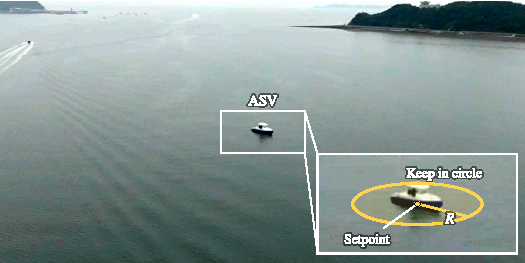
\includegraphics[width=\linewidth]{figures/fig_site.pdf}
\figph{Fig. 7 placeholder. Aerial view of the experimental site with the setpoint, the keep in circle, the prevailing wind direction during the trials, and a photograph of the vessel on station.}{4.5cm}
\caption{Experimental site and setpoint. \pending{Site, date, and wind conditions to be stated.}}
\label{fig_site}
\end{figure}

\subsubsection{Onboard Implementation}\label{sec_onboard}

The controller runs as a ROS~2 node on the control PC of Fig.~\ref{fig_vessel}. The position, heading, and body rates are estimated by an extended Kalman filter at 10~Hz from the measurements of the GPS and the AHRS of Table~\ref{tab_boat}. At each control period the node assembles the augmented state from the latest estimate, the commanded gear, and a software timer that mirrors the PLC lock, evaluates the task policy, the critic, and the shield, and publishes the steering command and the gear request to the PLC. Inference of the three networks takes \pending{TBD} ms per step on the control PC, well within the control period. The PID and NMPC baselines of Section~\ref{sec_baselines} run in the same node structure and differ only in the policy evaluation block, so that all three controllers share the same state estimate, control period, actuation interfaces, and dwell enforced by the PLC.

\subsection{Experimental Results}\label{sec_exp}

The field validation of the proposed controller against the PID and NMPC baselines is reported here. Only the runs designated by the authors as the official trials are reported, and every quantitative entry is pending their designation.

\subsubsection{Comparison With Baselines}\label{sec_exp_comp}

Fig.~\ref{fig_traj} shows the trajectories of the three controllers in the setpoint frame together with the keep in circle, and Fig.~\ref{fig_time} shows the time histories of the distance to the setpoint, the certified value, the gear level and its timer, and the shield flag for the proposed controller, together with the distance and gear histories of the baselines. Table~\ref{tab_field} summarizes the field metrics, which are the same as in Section~\ref{sec_sim_closed} with the addition of the realized disturbance level discussed below.

\begin{figure}[!t]
\centering
%\includegraphics[width=\linewidth]{figures/fig_traj.pdf}
\figph{Fig. 8 placeholder. Trajectories in the setpoint frame for B1, C1, and the proposed controller, with the keep in circle, the heading indicated along the trajectory, and the wind direction.}{5cm}
\caption{Field trajectories in the setpoint frame with the keep in circle of radius $R$. \pending{Designated runs to be inserted.}}
\label{fig_traj}
\end{figure}

\begin{figure}[!t]
\centering
%\includegraphics[width=\linewidth]{figures/fig_time.pdf}
\figph{Fig. 9 placeholder. Time histories for the proposed controller. Panels for the distance to the setpoint with the radius R, the certified value with the margin tau, the gear level with the timer, and the shield flag. Overlaid distance and gear histories of B1 and C1.}{6cm}
\caption{Time histories of the distance to the setpoint, the certified value, the gear level and timer, and the shield flag in the field. \pending{Designated runs to be inserted.}}
\label{fig_time}
\end{figure}

\begin{table}[!t]
\renewcommand{\arraystretch}{1.35}
\caption{Field Metrics on the Designated Runs}
\label{tab_field}
\centering
\footnotesize
\begin{tabular}{lccc}
\toprule
Metric & B1 & C1 & \textbf{Proposed} \\
\midrule
Run duration (s) & \pending{TBD} & \pending{TBD} & \textbf{\pending{TBD}} \\
Mean distance (m) & \pending{TBD} & \pending{TBD} & \textbf{\pending{TBD}} \\
RMS distance (m) & \pending{TBD} & \pending{TBD} & \textbf{\pending{TBD}} \\
Max distance (m) & \pending{TBD} & \pending{TBD} & \textbf{\pending{TBD}} \\
Time inside disk (\%) & \pending{TBD} & \pending{TBD} & \textbf{\pending{TBD}} \\
Switches per minute & \pending{TBD} & \pending{TBD} & \textbf{\pending{TBD}} \\
Max excursion in lock (m) & \pending{TBD} & \pending{TBD} & \textbf{\pending{TBD}} \\
Shield rate (\%) & n/a & n/a & \textbf{\pending{TBD}} \\
Time per step (ms) & \pending{TBD} & \pending{TBD} & \textbf{\pending{TBD}} \\
Realized disturbance to bound & \pending{TBD} & \pending{TBD} & \textbf{\pending{TBD}} \\
\bottomrule
\end{tabular}
\end{table}

The comparison is again read from the weakest to the proposed controller. The PID controller B1 held station with a mean distance of \pending{TBD}~m and left the disk \pending{TBD} times, and it shifted the gear \pending{TBD} times per minute, each shift opening a lock during which the distance grew by up to \pending{TBD}~m. The NMPC controller C1 held station with a mean distance of \pending{TBD}~m and \pending{TBD} excursions, with \pending{TBD} shifts per minute and a solve time of \pending{TBD}~ms per step. The proposed controller held station with a mean distance of \pending{TBD}~m, remained inside the disk for \pending{TBD} of the run, shifted \pending{TBD} times per minute, and triggered the shield in \pending{TBD} of the steps. These results would demonstrate that the certified controller transfers to the vessel without retraining and holds the disk against the real environmental load with fewer gear shifts than the baselines, \pending{to be stated once the designated runs are analyzed}.

\subsubsection{Discussion}\label{sec_exp_disc}

Three observations deserve comment. First, the behavior during locked intervals is the direct field evidence for the formulation of Section~\ref{sec_family}. In Fig.~\ref{fig_time} the distance to the setpoint should rise during each lock and recover after the timer expires, and the certified value should dip at the moment of a shift and recover with the timer, which is the signature of a value that reserves margin for the lock. The maximum excursion during locks in Table~\ref{tab_field} quantifies this reserve, and its comparison across controllers shows which of them opens locks at the wrong moments. \pending{Observed behavior to be described from the designated runs.}

Second, the shield interventions mark the moments at which the task policy proposed an action whose certified value fell below the margin. Because the task policy is trained under the floored Lagrangian penalty of \eqref{eq_lagrange}, interventions are expected to be rare and to occur near the boundary of the disk, typically when the task policy would request a shift that opens a lock while the vessel is being pushed outward. \pending{Intervention count and locations to be described.}

Third, the real disturbance encountered in the field is not a worst case adversary, and this is a strength of the deployment rather than a limitation of the validation. The realized disturbance during the trials, estimated from the drift during neutral locks and from the residual of the state estimate, amounted to \pending{TBD} of the bound \eqref{eq_wbox}. The certified margin that the controller reserved for the worst case was therefore only partly consumed, and the unconsumed part acted as a reserve against unmodeled effects such as wave induced motion, estimation error, and actuator timing jitter. A controller certified against the worst case therefore does not merely survive the field, it survives with a quantified reserve, which is the property one wants from a safety layer on a vessel that will meet stronger winds than those of the trial days.

\section{Conclusion}\label{sec_conclusion}

This article treated the gear shift dwell of a sterndrive vessel as a constraint on one player of the safety game rather than as a scheduling restriction, so that the safe set for weathervaning station keeping became a family indexed by the elapsed dwell, with the neutral lock as its most severe member. Promoting the gear and its timer to the state preserved the contraction of the discounted backup and allowed the dwell indexed value to be learned by a one step adversarial scheme with legality masking. Simulation showed that a certificate which ignores the dwell reports safety that does not exist, and the field trials showed the certified margin acting as a reserve against the real environmental load.

Two limitations bound these claims. First, the guarantees hold at the operator level, and no approximation bound is claimed for the neural representation. The deployed certificate is a margin shifted level set verified by adversarial Monte Carlo audit, which is evidence rather than proof. Second, the field validation covers a single dwell channel. The formulation extends to several channels at the price of notation only, and the bow thruster of the vessel is the natural next channel, but its verification burden grows with the number of channels and has not been exercised in the field. Addressing these limitations, together with the integration of wind measurements into the task policy, is the subject of future work.

\appendix[Proof of Lemma 1]

The proof of \cite[Theorems~2 and~3]{li2023cdc}, which itself builds on the discounted construction of \cite{fisac2019}, establishes contraction and monotonicity of the backup using only the following structural facts. The instantaneous term $(1-\gamma_h)h$ is fixed, the outer minimum with $h$ is nonexpansive, the minimization over $d \in \calW$ is nonexpansive, and the maximization over the admissible action set is nonexpansive, which requires only that the admissible set be nonempty and compact at every state. It does not require the admissible set to be constant across states. Under \eqref{eq_legal} the set $C(\xi)$ is nonempty for every $\xi$, since holding the current gear is always legal, and compact as the product of a finite set and a compact interval. Therefore, writing $(\Phi V)(\xi) = \max_{c \in C(\xi)} \min_{d \in \calW} V(F(\xi,c,d))$, for bounded $V$ and $V'$,
\begin{equation}
\bigl| (\Phi V)(\xi) - (\Phi V')(\xi) \bigr| \le \|V - V'\|_\infty \quad \text{for all } \xi \in \Xi,
\end{equation}
and composing with the outer structure of \eqref{eq_backup} gives
\begin{equation}
\|\calT_h V - \calT_h V'\|_\infty \le \gamma_h \|V - V'\|_\infty .
\end{equation}
Monotonicity is inherited term by term, since each of the operations above preserves the pointwise order. The Banach fixed point theorem on the complete space of bounded functions on $\Xi$ yields the unique bounded fixed point $V_h$. For robust invariance, let $V_h(\xi) \ge 0$ and let $c^\star \in C(\xi)$ attain the maximum in \eqref{eq_backup}, which exists by compactness. The fixed point equation gives $\min\{h(\xi), \min_{d} V_h(F(\xi, c^\star, d))\} \ge V_h(\xi) \ge 0$ after rearrangement, because $V_h(\xi) \le h(\xi)$ holds identically from the structure of \eqref{eq_backup}. Hence $h(\xi) \ge 0$ and $V_h(F(\xi, c^\star, d)) \ge 0$ for every $d \in \calW$, so the greedy legal action keeps the successor in $\calS$ for every disturbance, and the greedy policy belongs to $\Pi_C$ by construction. This is robust invariance of $\calS$ under dwell constrained admissible policies. No step of the argument counts the switching channels, which gives Remark~\ref{rem_channels}. $\blacksquare$

\bibliographystyle{IEEEtran}
\bibliography{references}

\biography{kiyong_park.png}{Kiyong Park}{received the B.S. degree in mechanical engineering from the Korea Advanced Institute of Science and Technology (KAIST), Daejeon, South Korea, in 2022. He is currently pursuing the integrated M.S. and Ph.D. degree in mechanical engineering with KAIST, Daejeon, South Korea. His research interests include model predictive control, disturbance observers, and control of autonomous surface vessels.}

\biography{jinwhan_kim.png}{Jinwhan Kim}{received his B.S. and M.S. degrees in Naval Architecture and Ocean Engineering from Seoul National University and the Ph.D. degree in Aeronautics and Astronautics from Stanford University. He is currently a professor of Mechanical Engineering at Korea Advanced Institute of Science and Technology (KAIST), Daejeon, South Korea.}

\end{document}
